\chapter{实验测试}\label{evaluation}

我们用900 LoC的\texttt{CUDA C++}实现了ko-Sched框架\footnote{实现代码可在\url{https://github.com/ryanyuan-yyr/ko-Sched}获取。},并实现了4个用于测试的可分割内核。在本章节,我们会展示使用ko-Sched指导带来的程序性能提升、ko-Sched使用的算法对GPU架构的通用性及搜索算法的高效性。本章涉及的所有实验在运行前均进行了充分的预热。

\section{实验环境}\label{exp-env}

\begin{table}[htbp]
    \caption{实验涉及的GPU硬件}
    \label{table:exp-env}
    \begin{tblr}{
        colspec = {rX[c,m]X[c,m]X[c,m]X[c,m]},
        hlines,
        vlines,
        }
        \hline
        \emph{NVIDIA GeForce GPU}   & \textbf{MX250}                                       & \textbf{RTX 2080Ti}                           & \textbf{RTX 3080}                             & \textbf{RTX 3090}                             \\
        \hline
        \emph{\#MP(MultiProcessor)} & $3$                                                  & $68$                                          & $68$                                          & $82$                                          \\
        \emph{\#CUDA cores}         & $384$                                                & $4352$                                        & $8704$                                        & $10496$                                       \\
        \emph{L2 cache size}        & $0.5$ MB                                             & $5.5$ MB                                      & $5$ MB                                        & $6$ MB                                        \\
        \emph{Max \#threads / MP}   & 2048                                                 & 1024                                          & 1536                                          & 1536                                          \\
        \emph{\#reg / block}        & 65536                                                & 65536                                         & 65536                                         & 65536                                         \\
        \emph{Shared mem / MP}      & $96$ KB                                              & $64$ KB                                       & $100$ KB                                      & $100$ KB                                      \\
        \emph{Global Memory}        & $1.95$ GB                                            & $10.76$ GB                                    & $10$ GB                                       & $23.69$ GB                                    \\
        \emph{Host CPU}             & Intel(R) Core(TM) i7-10510U CPU @ 1.80GHz   2.30 GHz & Intel(R) Xeon(R) Platinum 8255C CPU @ 2.50GHz & Intel(R) Xeon(R) Platinum 8255C CPU @ 2.50GHz & Intel(R) Xeon(R) Platinum 8350C CPU @ 2.60GHz \\
        \hline
    \end{tblr}
\end{table}

本文的实验涉及到4种GPU硬件,如\autoref{table:exp-env}所示。此外,我们将CUDA Samples SDK\cite{cuda_samples}中选取的3个测试程序和cCUDA\cite{8853389}使用的\texttt{sqrt\_pow}内核改写为使用ko-Sched框架的内核可分割版本,分别是:

\begin{description}
    \item[\texttt{matrix\_mul} (\texttt{mm})] 矩阵乘法内核,选取自CUDA Samples。将矩阵分块为$\texttt{BLOCK\_SIZE}\times\texttt{BLOCK\_SIZE}$大小的子矩阵,每个子矩阵从global memory加载至shared memory后进行子矩阵乘法运算,最后复制回global memory。
    \item[\texttt{vec\_add} (\texttt{va})] 矢量加法内核,选取自CUDA Samples。实现loop unrolling优化,每个thread负责矢量的连续若干个元素的运算。
    \item[\texttt{matrix\_transpose} (\texttt{mt})] 矩阵转置内核,选取自CUDA Samples。以tiling的方式实现,每个thread负责若干个元素的复制。
    \item[\texttt{sqrt\_pow} (\texttt{sp})] 一个运算密集型内核,选取自cCUDA\cite{8853389}的实现。每个线程进行大量的平方根和指数运算。
\end{description}

\section{Ko-Sched实现的性能提升}

本节将展示ko-Sched框架带来的性能提升。我们将对\texttt{mm}、\texttt{va}、\texttt{mt}和\texttt{sp}这4个内核间的组合进行测试,分别运行使用ko-Sched框架的可分割版本和作为baseline的未分割原始版本,比较两者的性能。对于原始版本,两个内核将在同一CPU线程的2个stream分别启动。对于可分割版本,我们将使用ko-Sched框架将两个内核分割为若干个子内核,同一内核的子内核在一个stream中启动。

\begin{figure}[htbp]
    \centering
    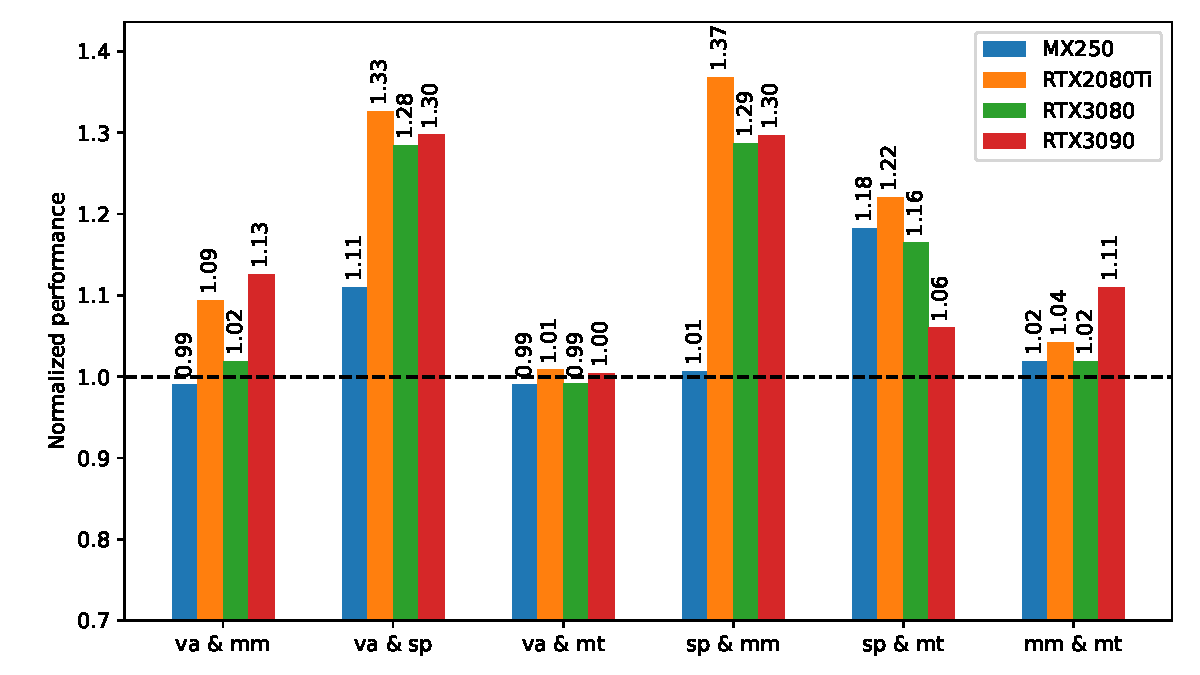
\includegraphics[width=\linewidth]{evaluation/perf-eval-diff-dev.pdf}
    \caption{在不同GPU上ko-Sched相对于未分割版本的性能。注意y轴的范围从0.7开始。}
    \label{perf-eval-diff-dev}
\end{figure}

\autoref{perf-eval-diff-dev}展示了使用ko-Sched计算得的参数进行kernel分割所得到的性能提升。图中展示了各测试程序组合在不同GPU硬件下相对于baseline的性能。可以看到,ko-Sched框架在绝大部分情形下带来了性能提升,平均提升达到$12.5\%$,在部分组合下甚至能达到$30\%$。这是因为ko-Sched框架能够将两个内核的计算任务同时派发给设备,提高GPU硬件的利用率。此外,我们还可以看到ko-Sched框架在不同的GPU硬件上均能带来性能提升,这说明ko-Sched框架的算法对GPU架构具有通用性。

\texttt{va}与\texttt{mt}的组合在所有GPU硬件上均未表现出明显的性能提升。这是因为\texttt{va}与\texttt{mt}均属于内存密集型应用,二者瓶颈均在内存操作上,因此将二者并行执行并不能提高性能。cCUDA\cite{8853389}提出了\emph{Kernel Mix Intensity}(KMI)指标用于将内核分为计算密集型和内存密集型。他们的工作同样指出\texttt{va}与\texttt{mt}同属于内存密集型应用。在他们的实验中,\texttt{va}与\texttt{mt}的组合也未表现出明显的性能提升。\texttt{va}与\texttt{sp}的组合在所有GPU硬件上均表现出较明显的性能提升。这是因为\texttt{va}属于内存密集型应用,\texttt{sp}属于计算密集型应用,二者的瓶颈不同,内存指令执行与计算指令执行可以互相隐藏,从而提高性能。这两个例子说明为实现性能提升需谨慎选择并行的内核组合。

在部分测试程序的组合中,不同GPU硬件的表现有较大差异。例如,在\texttt{sp}和\texttt{mm}的组合中,MX250几乎未表现出性能提升,而其余GPU的性能提升达到了近30\%。这种差异并非仅仅由GPU性能高低导致。例如,在\texttt{sp}和\texttt{mt}的组合中,综合性能最佳的RTX 3090表现出的性能提升最低。这种差异源于同一测试程序在不同GPU上表现出的特征不同,故为达到最佳性能需要针对不同GPU进行参数计算。Ko-Sched的算法能够根据不同GPU的特征计算出不同的参数,达到较好的效果。

\begin{figure}[htbp]
    \centering
    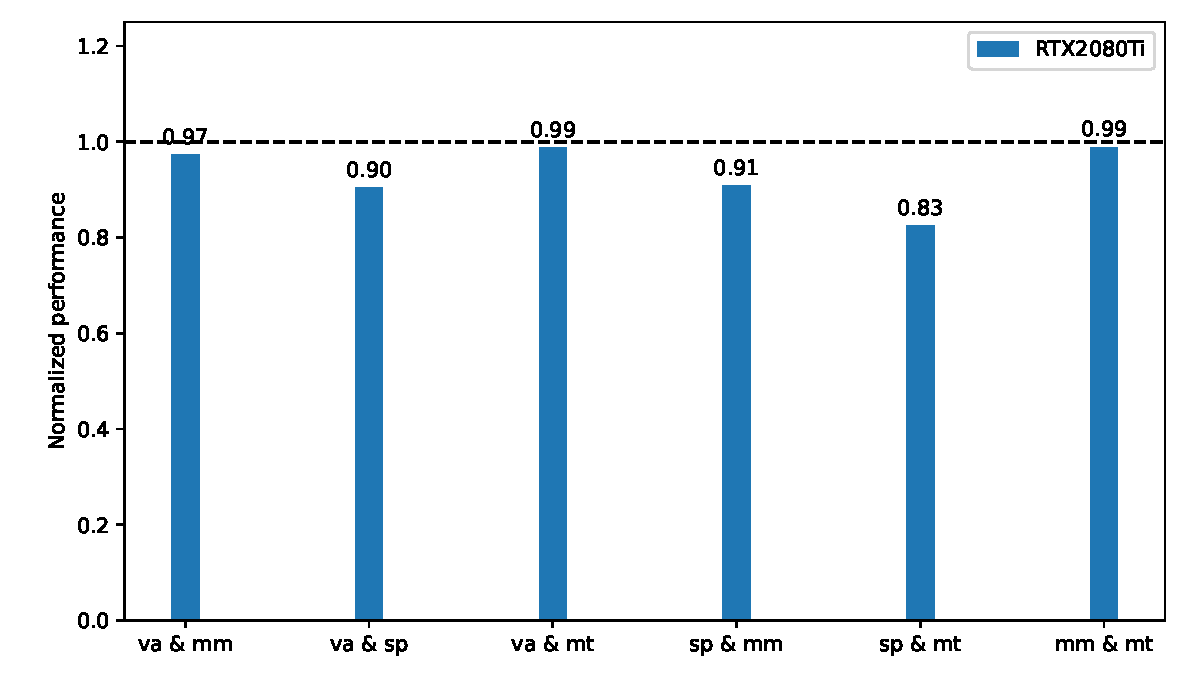
\includegraphics[width=\linewidth]{evaluation/perf-eval-compared-to-opt.pdf}
    \caption{ko-Sched相对于最佳分割参数下的性能。}
    \label{perf-eval-cmp-opt}
\end{figure}

为了说明ko-Sched算法所得结果的最优性,我们在RTX 2080Ti硬件上测试了大量的分割参数组合下的程序性能\footnote{我们测试了所有满足子内核数目大于3且子内核大小至少为\autoref{eq:searching:stepsize}所确定数值的参数组合},找到了其中性能最佳的参数组合。我们将ko-Sched算法所得结果与这个参数下的性能进行比较,结果如\autoref{perf-eval-cmp-opt}所示。可以看到,ko-Sched算法所得结果的性能与最优结果的性能相差不大,平均达到了最佳性能的$93.14\%$。这说明ko-Sched算法所得结果的最优性。

\section{执行时间估算的效果}\label{exp-est}

\begin{figure}[htbp]
    \centering
    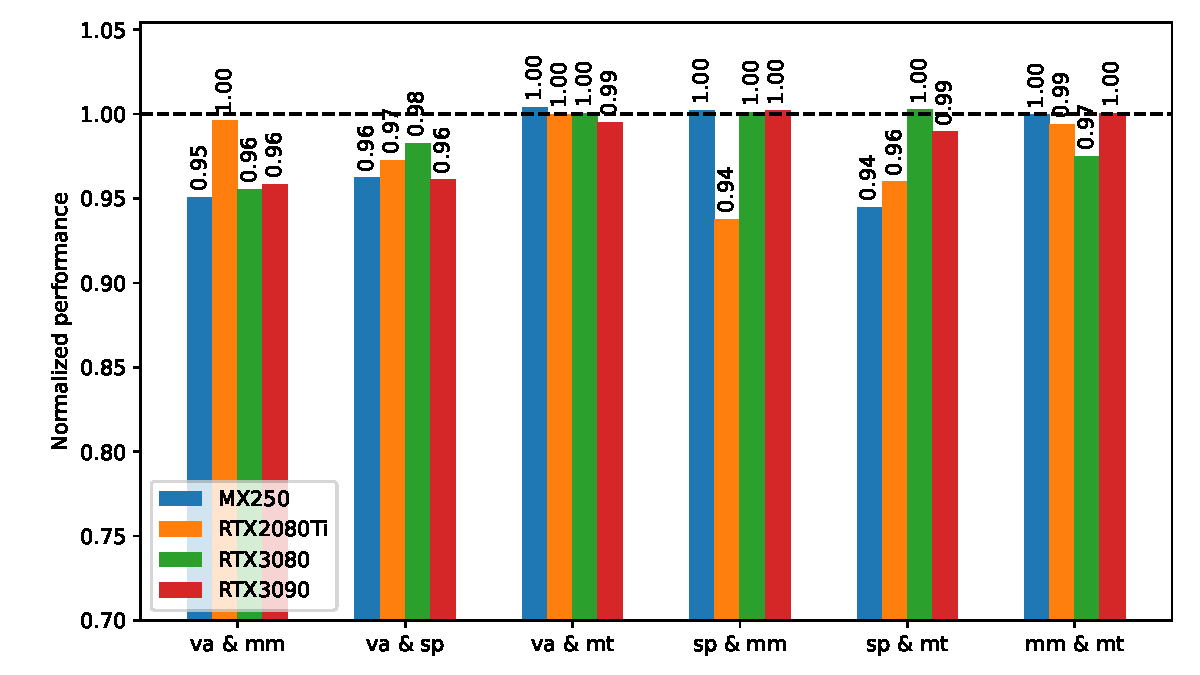
\includegraphics[width=\linewidth]{evaluation/perf-eval-compared-to-nonsampling.pdf}
    \caption{ko-Sched相对于ko-Sched'的性能。注意y轴的范围从0.7开始。}
    \label{perf-eval-compared-to-nonsampling}
\end{figure}

\autoref{chapter:design-implementation}\autoref{sec:profile}提到,ko-Sched在搜索时仅执行部分subkernel样本并以此估计整个kernel的执行时间。然而,由于估算的执行时间不准确,据此得到的搜索结果可能劣于使用准确测量得到的搜索结果。本节将展示通过估算取得的结果依然能够达到较好的性能。

我们实现了ko-Sched的变种,\emph{ko-Sched'},其在搜索时不进行subkernel取样,而是直接执行所有subkernel并记录执行时间。相较于ko-Sched, ko-Sched'获得了准确的执行时间,因此最终得到的结果更加准确。我们将ko-Sched的结果与ko-Sched'的结果进行比较,结果如\autoref{perf-eval-compared-to-nonsampling}所示。可以看到,ko-Sched的结果与ko-Sched'的结果相差不大,在所有GPU硬件和测试程序组合下平均达到了ko-Sched'结果的$98.12\%$。这说明ko-Sched的执行时间估算能够在不影响性能的情况下加速搜索过程。
